\newpage
\section{Architettura dei container}
La progettazione del sistema \textit{DIPReader} è stata guidata dai principi di modularità, scalabilità e manutenibilità, con l'obiettivo di creare un'architettura che possa evolversi nel tempo e adattarsi a nuove esigenze e normative AGID.\\
\begin{figure}[H]
    \centering
    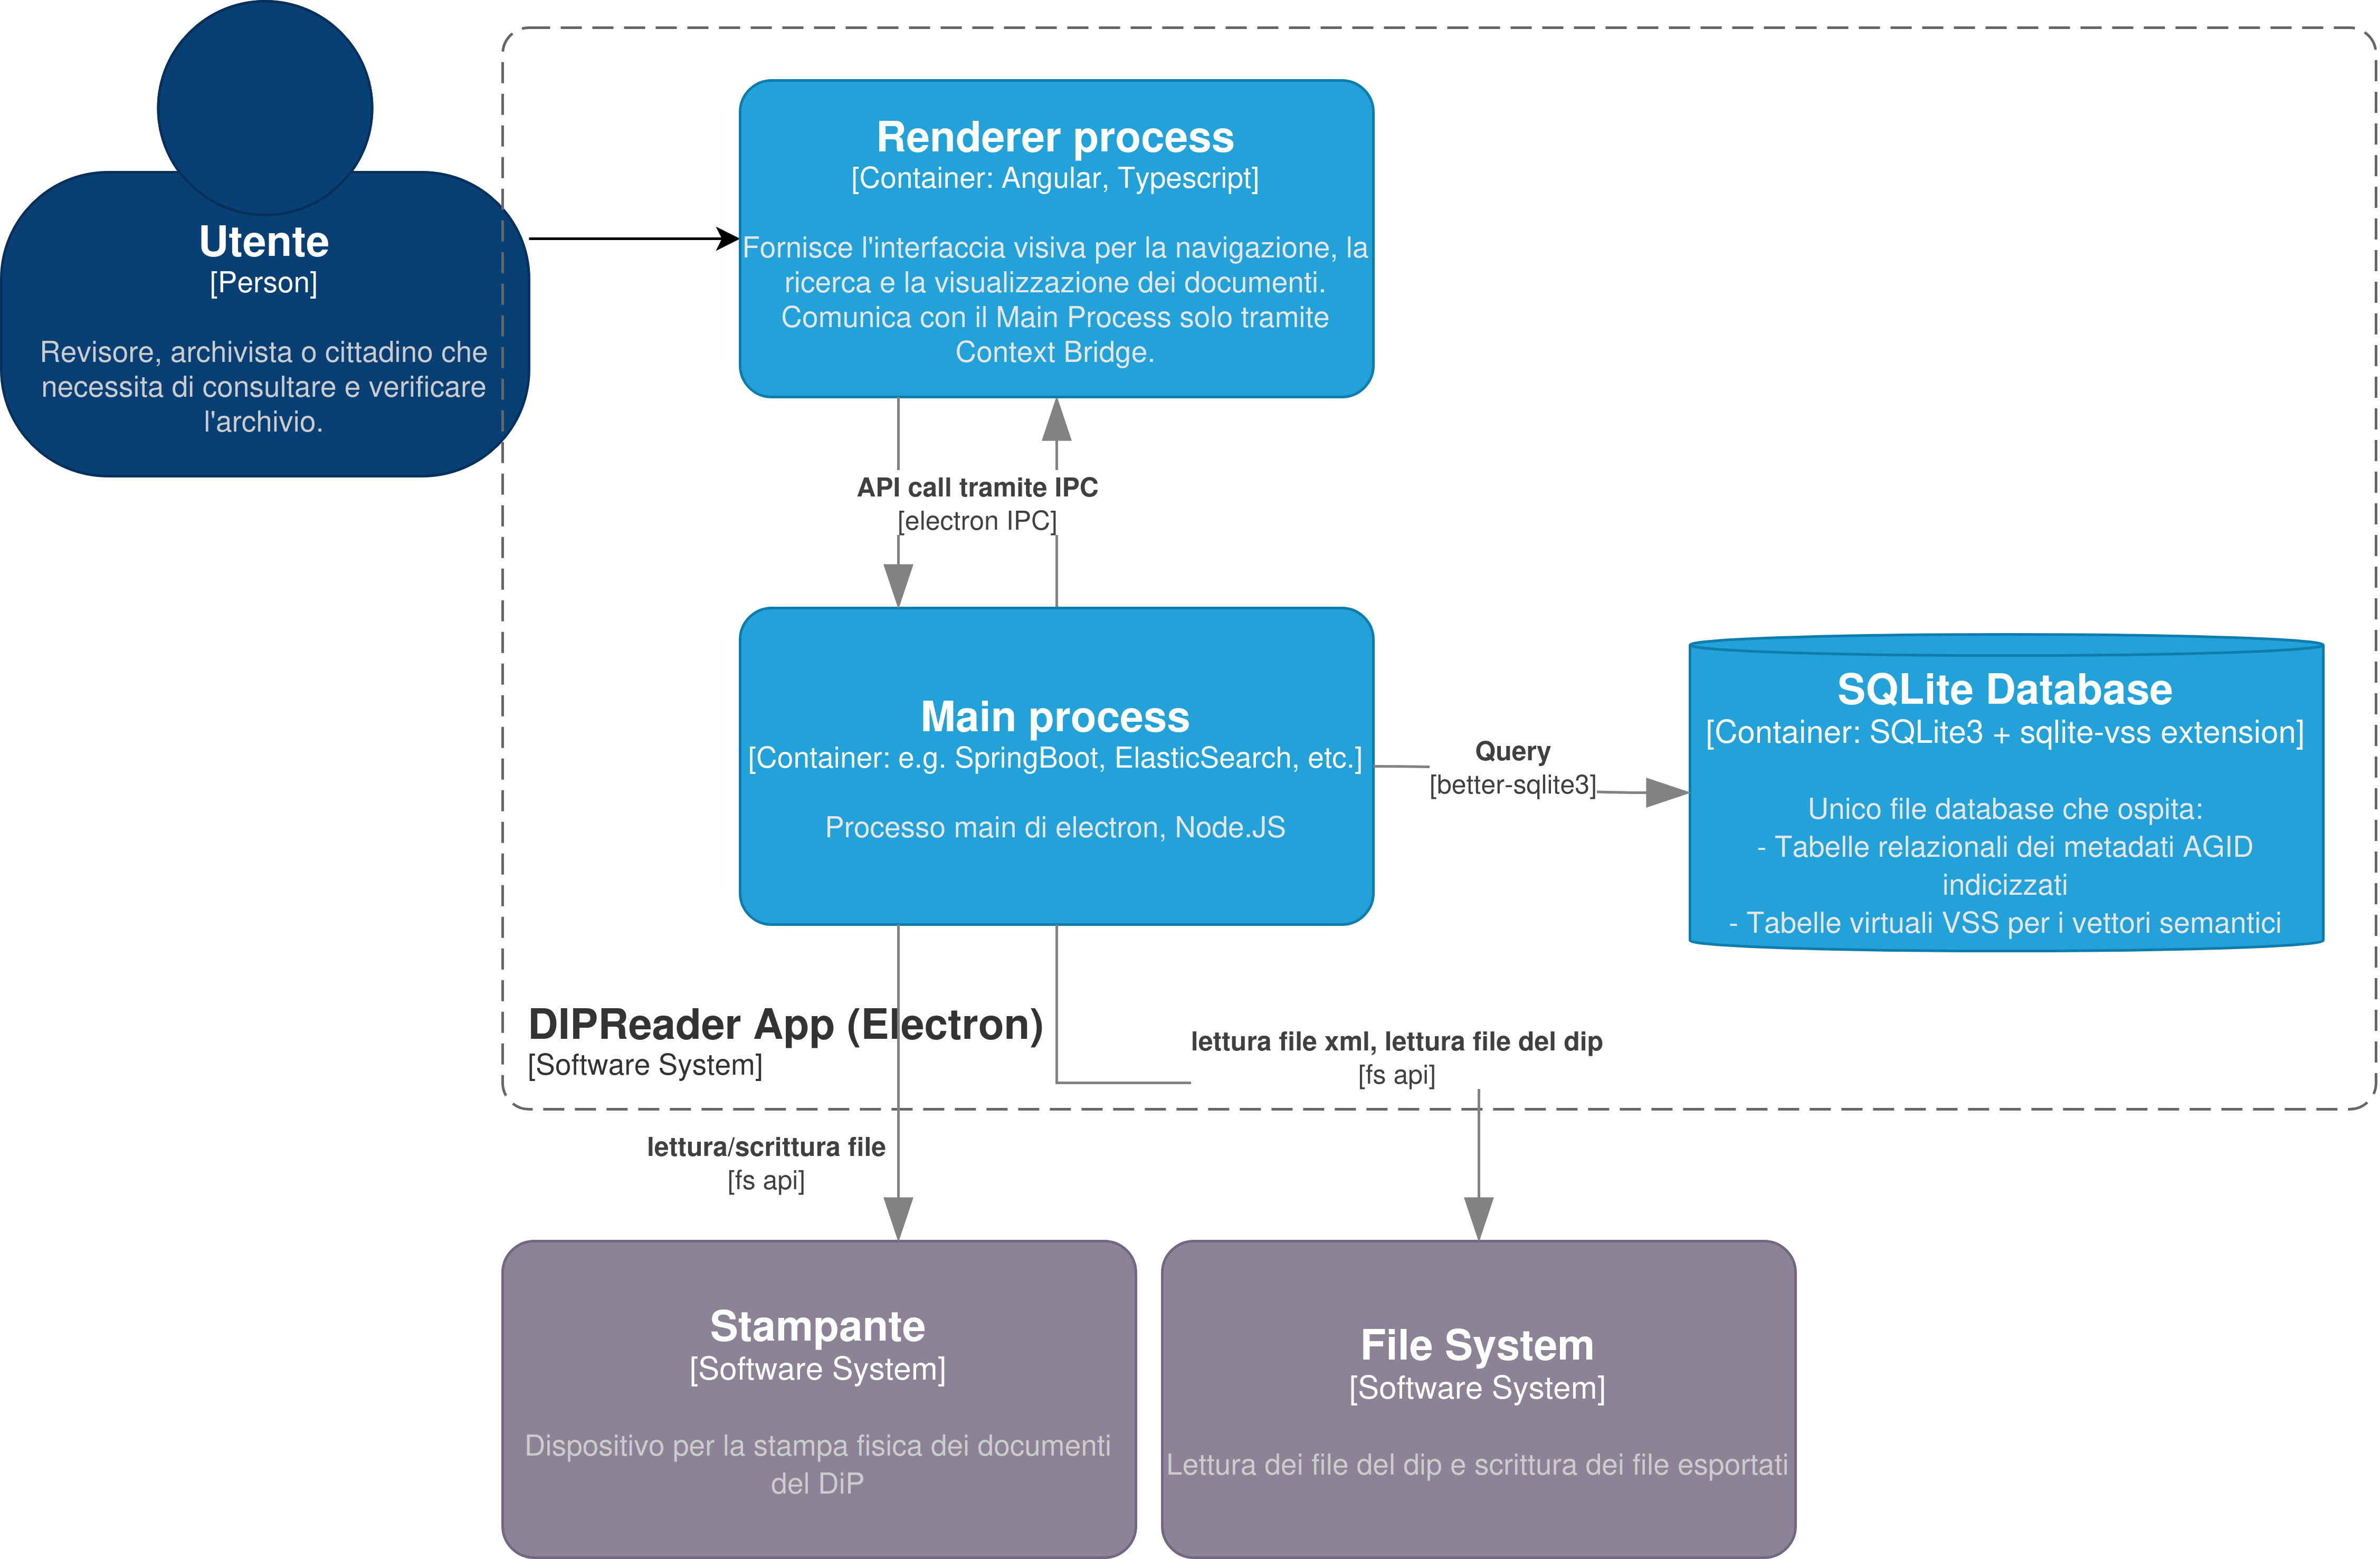
\includegraphics[width=1\textwidth]{../../assets/outDiagrammiST/DiagrammaC2(1).png}
        \caption{Diagramma C2 - Container del sistema \textit{DIPReader}}
    \label{fig:C2_container}
\end{figure}

\subsection{Renderer}
\subsubsection{Struttura architetturale}
Il container \textit{Renderer} è responsabile della presentazione dell'interfaccia utente e dell'interazione con l'utente. 
Il processo renderer ospita l'applicazione Angular, eseguita dal motore Chromium di Electron. Il frontend è sviluppato come SPA (Single Page Application) e segue un'architettura a componenti, con una chiara separazione tra logica di presentazione e logica di coordinamento. È inoltre applicato il pattern Smart and Dumb Components, che separa la logica di orchestrazione dalla presentazione pura.\\
Infine, essendo l'applicazione sviluppata in Angular, adotta il pattern MVVM (Model View ViewModel) per la gestione della UI.
\subsubsection{Relazione con i principi SOLID}
\begin{itemize}
    \item \textbf{SRP:} ogni componente ha una sola responsabilità.
    \item \textbf{OCP:} nuovi componenti possono essere aggiunti estendendo i contratti esistenti.
    \item \textbf{LSP e ISP:} i layer dipendono da interfacce coese e sostituibili. 
    \item \textbf{DIP:} Sono iniettati i token delle interfacce dei servizi, non le implementazioni concrete.
\end{itemize}

\subsection{Main}
\label{sec:container:main}

\subsubsection{Ruolo architetturale}
Il container \textit{Main} ospita la logica backend e costituisce il punto di orchestrazione tra IPC, use case applicativi e persistenza su SQLite.
Le responsabilita principali sono la registrazione degli handler IPC, l'implementazione della business logic e il bootstrap iniziale dei dati indicizzati.
In particolare, l'architettura del main process è stata organizzata in maniera tale da definire solamente le entità di un pacchetto DiP, gestendo invece i metadati in maniera generica. Questo permetterà in un futuro di evolvere il sistema per supportare nuovi tipi di schema di metadati, senza dover modificare o aggiungere nessuna componente o entità al backend.

\subsubsection{Layer architetturali}
\begin{enumerate}
    \item \textbf{IPC Adapter:} boundary verso renderer, gestione canali, mapping DTO.
    \item \textbf{Use Case:} business logic layer, utilizza servizi e porte outbound per ottenere il risultato.
    \item \textbf{Outbound port:} layer di astrazione per l'interazione con servizi esterni.
    \item \textbf{Outbound adapter:} implementazione concreta delle porte verso p.e. database o filesystem.
    \item \textbf{DAO:} query SQL concrete, ricostruzione entity da righe.
    \item \textbf{Mapper:} trasformazione DTO $\leftrightarrow$ Entity $\leftrightarrow$ Persistence.
    \item \textbf{Entity / Value Objects:} modello di dominio.
\end{enumerate}

\subsubsection{Relazione con i principi SOLID}
\begin{itemize}
    \item \textbf{SRP:} ciascun componente ha un solo motivo per cambiare: ciascuna classe ha una responsabilità ben definita e limitata. Sinonimo di coesione: un classe è coesa se le classi client che la utilizzano usano tutti i metodi della classe.
    \item \textbf{OCP:} nuovi use case o adapter possono essere aggiunti estendendo i contratti esistenti.
    \item \textbf{LSP e ISP:} i layer dipendono da interfacce coese e sostituibili.
    \item \textbf{DIP:} le concretizzazioni (adapters) dipendono da astrazioni (porte), non viceversa.
\end{itemize}

\subsubsection{Bootstrap e indicizzazione}
\noindent
\textbf{DatabaseBootstrap.ts} (avvio):
\begin{enumerate}[labelwidth=0.8cm,leftmargin=1cm]
    \item Ricrea database zero.
    \item Applica schema.
    \item Chiama \codeword{IndexDip.execute(dipPath)}.
\end{enumerate}

\subsubsection{Wiring runtime e registrazioni}
\noindent
Durante l'avvio dell'applicazione electron, \codeword{main.ts} esegue:

\begin{enumerate}[labelwidth=0.8cm,leftmargin=1cm]
    \item bootstrap database tramite \codeword{ApplicationBootstrapAdapter}
    \item registrazione token runtime \codeword{DIP\_PATH\_TOKEN}
    \item registrazione adapter IPC (es. \codeword{BrowsingIpcAdapter}, \codeword{CheckIntegrityIpcAdapter})
\end{enumerate}